\subsection{Particelle doppie}

L'uso dell'ADC ci consente di avere la distribuzione dell'energia persa dai raggi cosmici nell'attraversare i nostri rivelatori. Ci aspettiamo allora di osservare una distribuzione con moda doppia nel caso in cui ci sia un passaggio frequente di 2 particelle nello stesso momento. Nel caso in cui l'arrivo di particelle doppie non fosse predominante ma significativo rispetto al numero di eventi totali ci aspetteremmo una distribuzione con 2 picchi in cui il picco più basso ha valore doppio (in ascissa) rispetto a quello più alto.

Per eseguire questa misura studiamo lo spettro energetico in funzione della soglia per una coppia di scintillatori: PM5 e PM4. Il PM5 è collegato all'ADC ed ha la soglia più bassa possibile (\SI{30}{mV}) in modo da poter misurare qualsiasi rilascio. La soglia del PM4 viene variata di volta in volta. \marginpar{aggiungere tabella?}  La nostra idea \marginpar{In realtà di Marco Stanislao Sozzi} è quella di eliminare il più possibile le particelle singole 
\marginpar{c'è bisogno di specificare che ``eliminare'' non significa distruggere i muoni ma fregarcene?}
in modo da vedere una percentuale predominante di particelle doppie nel caso il loro passaggio sia frequente.

Tutti gli istogrammi analizzati presentano un unico picco e la loro moda è rappresentata in \autoref{corre} in funzione della soglia.

\begin{figure}[h]
\centering
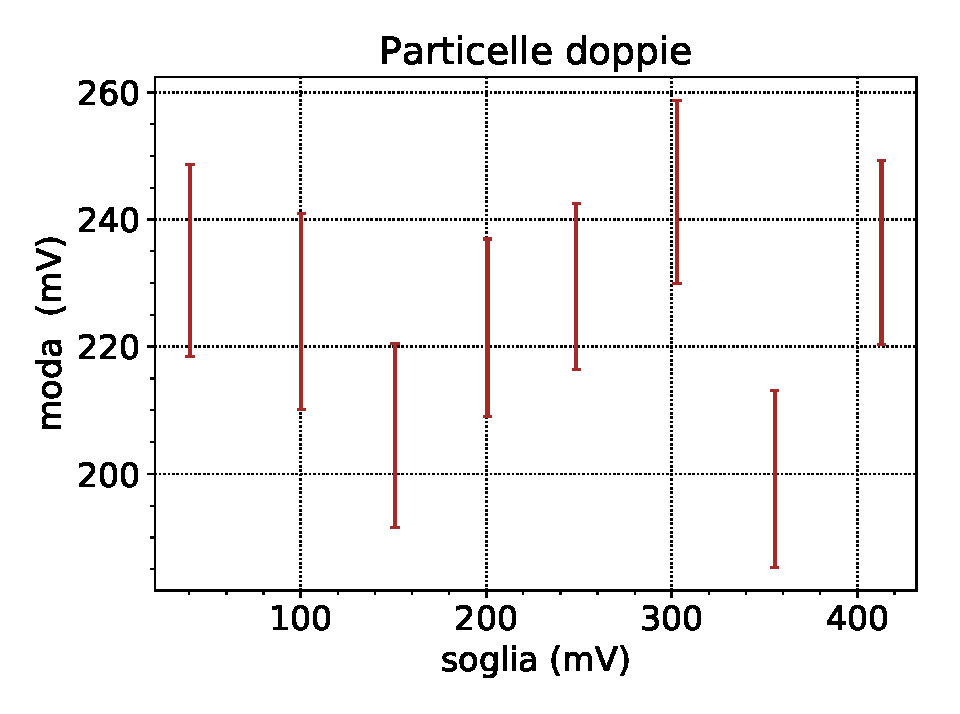
\includegraphics[width=10 cm]{doppie}
\caption{moda degli istogrammi in funzione della soglia del PM4.}
\label{corre}
\end{figure}

L'errore sul valore della soglia%
\footnote{Misurato nel test point con il tester.}
vale \SI{0.3}{mV} in quanto il valore letto sul tester fluttuava di tale quantità al variare del tempo. L'errore sulla moda è la semilarghezza del canale dell'istogramma.
Dalla \autoref{corre} è facile notare che l'andamento da noi ipotizzato non si è verificato. Se avessimo avuto a disposizione due ADC avremmo potuto analizzare le correlazioni temporali tra rilasci elevati di energia in due scintillatori diversi. Il passaggio simultaneo di due particelle potrebbe essere rivelato attraverso in riconoscimento  di rilasci elevati e simili (tra i due scintillatori) di energia.